\documentclass[conference]{IEEEtran}
\usepackage[top=3cm, bottom=2cm, left=2cm, right=2cm, columnsep=20pt]{geometry}
\usepackage{pdfpages}
\usepackage{graphicx}
\usepackage{etoolbox}
\apptocmd{\sloppy}{\hbadness 10000\relax}{}{}
% \usepackage[numbers]{natbib}
\usepackage[T1]{fontenc}
\usepackage{ragged2e}
\usepackage[french]{babel}
\usepackage{listings}
\usepackage{color}
\usepackage{soul}
\usepackage[utf8]{inputenc}
\usepackage[export]{adjustbox}
\usepackage{caption}
\usepackage{mathrsfs, amsmath}
\usepackage{amssymb}
\usepackage{float}
\usepackage{csquotes}
\usepackage{fancyhdr}
\usepackage{wallpaper}
\usepackage{siunitx}
\usepackage[indent]{parskip}
\usepackage{textcomp}
\usepackage{gensymb}
\usepackage{multirow}
\usepackage[hidelinks]{hyperref}
\usepackage{abstract}
\usepackage{subcaption}
\usepackage{tabularx}
\usepackage{biblatex}
\addbibresource{bibliographie.bib}

% \renewcommand{\abstractnamefont}{\normalfont\bfseries}
% \renewcommand{\abstracttextfont}{\normalfont\itshape}
\usepackage{titlesec}
% \titleformat{\section}{\large\bfseries}{\thesection}{1em}{}
% \titleformat{\subsection}{\normalsize\bfseries}{\thesubsection}{1em}{}
% \titleformat{\subsubsection}{\normalsize\bfseries}{\thesubsubsection}{1em}{}

\usepackage{xcolor}
\definecolor{codegreen}{rgb}{0,0.6,0}
\definecolor{codegray}{rgb}{0.5,0.5,0.5}
\definecolor{codepurple}{rgb}{0.58,0,0.82}
\definecolor{backcolour}{rgb}{0.95,0.95,0.92}
\lstdefinestyle{mystyle}{
    backgroundcolor=\color{backcolour},   
    commentstyle=\color{codegreen},
    keywordstyle=\color{magenta},
    numberstyle=\tiny\color{codegray},
    stringstyle=\color{codepurple},
    basicstyle=\ttfamily\footnotesize,
    breakatwhitespace=false,         
    breaklines=true,                 
    captionpos=b,                    
    keepspaces=true,                 
    numbers=left,                    
    numbersep=5pt,                  
    showspaces=false,                
    showstringspaces=false,
    showtabs=false,                  
    tabsize=2
}
\lstset{style=mystyle}

\usepackage[most]{tcolorbox}
\newtcolorbox{note}[1][]{
  enhanced jigsaw,
  borderline west={2pt}{0pt}{black},
  sharp corners,
  boxrule=0pt, 
  fonttitle={\large\bfseries},
  coltitle={black},
  title={Note:\ },
  attach title to upper,
  #1
}

\pagestyle{plain}
%----------------------------------------------------

\setlength{\parindent}{0pt}
\DeclareCaptionLabelFormat{mycaptionlabel}{#1 #2}
\captionsetup[figure]{labelsep=colon}
\captionsetup{labelformat=mycaptionlabel}
\captionsetup[figure]{name={Figure }}
\captionsetup[table]{name=Tableau}
\newcolumntype{Y}[1]{>{\Centering\hspace{0pt}\hsize=#1\hsize}X}
\newcommand{\inlinecode}{\normalfont\texttt}
\usepackage{enumitem}
\setlist[itemize]{label=\textbullet}

\begin{document}

%----------------------------------------------------
\title{Microscope\\
\large Travail préparatoire \\
PHS3910 -- Techniques expérimentales et instrumentation\\ 
Équipe L3}

\author{\IEEEauthorblockN{Émile Guertin-Picard}
\IEEEauthorblockA{2208363}
\and
\IEEEauthorblockN{Maxime Rouillon}
\IEEEauthorblockA{2213291}
\and
\IEEEauthorblockN{Marie-Lou Dessureault}
\IEEEauthorblockA{2211129}
\and
\IEEEauthorblockN{Philippine Beaubois}
\IEEEauthorblockA{2211153}
}

\maketitle

\textit{\textbf{Résumé} -- Modélisation préliminaire d'un microscope capable de déterminer la taille de 
particules. La magnification et la PSF d'une particule sont simulés. Son déplacement est simulé à l'aide du
mouvement brownien, et le coefficient de diffusion est extrait de la courbe du MSD de la particule. }
\section{Introduction}
Ayant reçu un contrat d'un gouvernement local nécessitant d'examiner les microparticules contaminantes proches d'une
usine, l'équipe est mandaté de concevoir un microscope capable de déterminer la taille de particules. En préparation à la conception
du produit final, une simulation du mouvement d'une particule, tel qu'elle serait perçue à travers le microscope, ainsi qu'une
analyse de son déplacement est développée. En simulant la magnification et la fonction d'étalement de la particule (\textit{PSF}), ainsi qu'en soumettant
celle-ci à un mouvement brownien, il est possible
de retrouver le coefficient de diffusion à partir de la pente de la courbe de son déplacement moyen au carré (\textit{MSD}).
La taille de la particule peut directement être extraite de ce résultat. Cette démarche préliminaire permettra
d'estimer l'erreur sur la taille en fonction de certains paramètres du système optique \textcolor{red}{lesquels???}.

\textcolor{red}{rajouter le résultat} Le rapport ci-contre expliquera en détail les méthodes de simulation utilisées pour obtenir 
les résultats souhaités, présentera les tailles et les erreurs respectives pour chaque ensemble de paramètres et développera les raisonnements
justifiants les choix de l'équipe.


\section{Méthodes \label{methodes}}
Le système optique utilisé pour la conception du microscope est illustré de manière simplifiée
dans la figure \ref{sys} ci-dessous.
\begin{figure}[H]
  \centering
  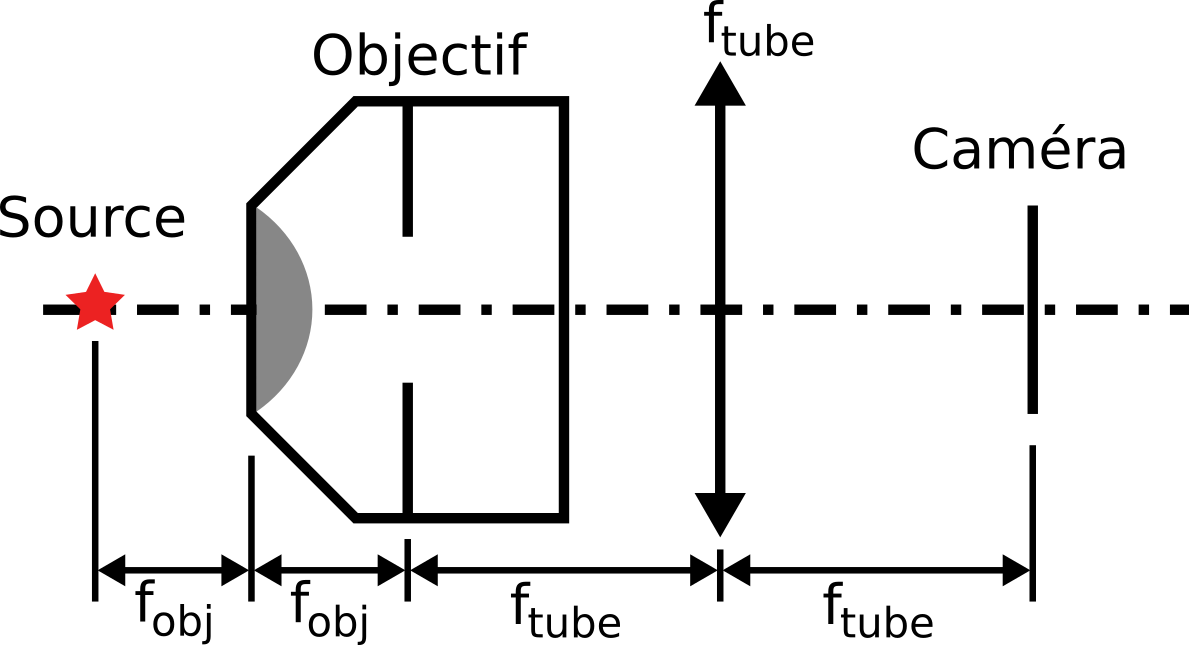
\includegraphics[scale=2.3]{systeme.png}
  \caption{Système optique simplifié du microscope.}
  \label{sys}
\end{figure}
Afin de simuler les observations et les analyses qui seront faites avec le microscope,
une modélisation du mouvement d'une particule a premièrement été effectué sur un scripte Python.
Pour les fins du projet, il a été décidé que de simuler une seule particule serait suffisant pour
évaluer les paramètres à optimiser \textcolor{red}{pk?}. En guise d'équivalence de la magnification réelle du microscope, 
une taille de pixel effective $P$ a eu besoin d'être posée. Le calcul de cette taille $P$ est obtenue à partir du grossissement $M$ de l'objectif ainsi qu'avec la
focale de la lentille de tube $f_{tube}$. Le grossissement est défini tel que :

\begin{equation}
  M = \frac{f_{tube}}{f_{obj}},
\end{equation}

où $f_{obj}$ est la longueur focale de la lentille objectif. Le grossissement $M$ connu des lentilles suit
un standard de la \textit{Royal Microscopical Society} (RMS) qui pose $f_{tube}$ à 160 mm
\textcolor{red}{source A}. Ainsi, pour avoir le grossissement réel $M_{r}$, il faut convertir avec la 
formule suivante :

% Source A : https://www.microscopyu.com/microscopy-basics/infinity-optical-systems

\begin{equation}
  f_{1}= \frac{160 \text{ mm} }{M} \Rightarrow M_{r} = \frac{f_{obj}M}{160 \text{ mm} }.
\end{equation}

La taille réelle d'un pixel de caméra $p_r$, d'une valeur de 3.45 µm pour la caméra Zelux CS165MU
mise à disposition pour ce contrat \textcolor{red}{source B}, peut être convertie en taille effective
avec le grossissement réel :

\begin{equation}\label{pixel}
  P = \frac{p_{r}}{M_{r}} = \frac{p_{r}\;160 \text{ mm}}{f_{obj}M}.
\end{equation}

Pour créer un environnement plus fidèle à la réalité, un fond de bruit
a été rajouté, où les photons émis suivent une distribution de Poisson avec \textit{np.random.poisson}. En raison de la diffraction 
causée par le système optique, la particule a due être simulée
telle qu'elle serait perçue par la caméra dans le montage réel. En fonction des composantes optiques utilisées,
la PSF (\textit{Point Spread Function}) de la particule sur le capteur est décrite par:
\begin{equation}
  PSF(r)=\left(\frac{2J_1(\frac{2\pi \text{NA}r}{\lambda})}{\frac{2\pi \text{NA}r}{\lambda}}\right)^2,
\end{equation}
où NA est l'ouverture numérique de l'objectif, $\lambda$ est la longueur d'onde de la lumière passant à travers
le microscope et r est la distance radiale par rapport à la position de l'émetteur \textcolor{red}{source procédurier}. Ici, $J_1$
est une fonction de Bessel. L'émission des photons dans le temps s'effectue selon une distribution de Poisson:
\begin{equation}
  P(X=k)=\frac{\lambda^k e^{-\lambda}}{k!},
\end{equation}
où $k$ est le nombre d'évènements et $\lambda$ est le nombre moyen d'évènements
survenus au cours d'un intervalle de temps $\Delta t$ (le temps d'acquisition). Numériquement, ceci correspond à effectuer un nombre de simulations
d'émission choisi avec \textit{np.random.poisson} et un $\lambda$ arbitraire \textcolor{red}{setté à cbn?}. La position de chaque photon
émis durant la simulation est déterminée à l'aide de la distribution de probabilité imposée par la fonction d'étalement 
de la particule ($PSF$).

Pour simuler le mouvement d'une particule, on utilise le principe du mouvement brownien.
C'est-à-dire que le centre d'une gaussienne est placé à la position exacte de la particule,
la gaussienne a l'écart-type suivant:
\begin{equation}
  \sigma = \sqrt{2D\Delta t} = \sqrt{2\left ( \frac{k_{B}T}{2\pi \eta r} \right )\Delta t},
\end{equation}
où $D$ est le coefficient de diffusion, $k_{B}$ la constante de Blozmann, T la température en Kelvin, $\eta$ la viscosité en $Pa\cdot s$, r le rayon de la particule en mètre et $\Delta t$ le temps entre chaque déplacement en secondes. 
Cette gaussienne permet de déterminer la probabilité de présence de la particule sur une position x et y, relativement proche de la position initiale, après un certain temps $\Delta t$.  Avec une fonction python, 
il est possible de placer la particule à sa nouvelle position en tenant compte de ces probabilités. Cette opération est repérée successivement pour observer finalement 
le déplacement de la particule, et est testé pour des particules de diamètre de 1 et 10 µm.


Après avoir simulé le mouvement d'une particule, l'analyse a pu être effectuée en utilisant une procédure similaire
à celle qui sera utilisée pour le système réel. Pour chaque image capturée lors de l'acquisition (définie par un temps d'acquisition $\Delta t$), un \textit{fit}
d'une gaussienne 2D a été effectuée avec la librairie \textit{lmfit}. La fonction gaussienne 2D est définie par:
\begin{equation}
  f(x,y)=A\cdot exp\left(-\left[\frac{(x-x_0)^2}{2\sigma_x^2}+\frac{(y-y_0)^2}{2\sigma_y^2}\right]\right)+B.
\end{equation}
\textcolor{red}{où $A$ est... }À partir de la fonction obtenue, les moyennes en $x$ et en $y$ ($x_0,y_0$) de la gaussienne sont obtenus
pour déterminer la position de la particule à cet instant. En effectuant ce processus pour chaque image de l'acquisition,
on a pu obtenir le déplacement général de la particule pour un certain lapse de temps.


Une fois chaque position obtenue, il est possible de trouver la valeur du coefficient de diffusion de la particule. 
Pour ce faire il est nécessaire d'effectuer le calcul du déplacement quadratique moyen. On réalise ce calcul en faisant la moyenne des déplacements de même intervalle. Par exemple, 
la première moyenne sera calculée avec toutes les distances séparant deux positions éloignées à intervalle de $\Delta t=1$. De la même manière, la deuxième moyenne sera calculée avec toutes les distances
entre deux point placés a $\Delta t=2$ d'intervalle. On peut modéliser ce calcul par la formule suivante: 
\begin{equation}
  MSD(d) = \frac{1}{N_{\Delta t}} \sum_{i=0}^{N_{\Delta t} - 1} \left( \mathbf{r}(i+\Delta t) - \mathbf{r}(i) \right)^2
\end{equation}
Avec $N_{\Delta t}$ qui est le nombre de pairs i disponible pour un intervalle $\Delta t$ et $\Delta t$ qui varient de 1 jusqu'au nombre de positions-1. 
Une fois les valeurs des MDS trouvés pour chaque déplacement de même intervalle, il est possible de généré un graphique 
des MDS en fonction de la valeur de l'intervalle $\Delta t$. Sur ce graphique, seuls les premiers points seront sélectionnés, c'est à dire pour des $\Delta t$ faible.
Cette procédure est nécessaire pour observée le réel comportement du mouvement, car plus $\Delta t$ est petit, plus il y a de paire de points disponible. 
Une fois que seuls les premiers points apparaissent sur le graphique, il est possible d'effectuer une régression linéaire sur
ces points, c'est la pente de cette régression qui donnera la valeur du coefficient de diffusion $D$ et la taille de la particule $r$ estimée par notre microscope :

\begin{equation}
  \langle MSD(t) \rangle = 4Dt + 4\sigma^{2}
\end{equation}

Les valeurs obtenues par cette procédure comportent toutes une incertitude. Pour commencer, l'incertitude sur chaque 
position x et y de chaque point est donné par l'écart type de sa gaussienne, cette incertitude est donc donnée par 
\begin{equation}
  \Delta x=\Delta y=\sigma 
\end{equation}
Une fois l'incertitude déterminée pour chaque valeur, on veut pouvoir déterminer l'incertitude sur chaque valeur de la MSD. 
Pour ce faire, on propage l'incertitude, par la formule suivante, de chaque position sur la valeur de la MSD  correspondante: 
\begin{equation}
  \alpha =A+B
\end{equation}
\begin{align*}
  A = \sqrt{
    \begin{aligned}
      &\left( 2(x(i+\Delta t) - x(i))\cdot \Delta x(i+\Delta t) \right)^2 \\
      &+ \left( 2(x(i+\Delta t) - x(i))\cdot \Delta x(i) \right)^2
    \end{aligned}
  }
\end{align*}
\begin{align*}
  B = \sqrt{
    \begin{aligned}
      &\left( 2(y(i+\Delta t) - y(i))\cdot \Delta y(i+\Delta t) \right)^2 \\
      &+ \left( 2(y(i+\Delta t) - y(i))\cdot \Delta y(i) \right)^2
    \end{aligned}
  }
\end{align*}

\begin{equation}
  \Delta MSD=\frac{1}{N_{\Delta t}}\sqrt{\sum_{0}^{N_{\Delta t}-1}\alpha }
\end{equation}
En sachant que $\left ( r(i+\Delta t)-r(i) \right )^{2}=\left ( x(i+\Delta t)-x(i) \right )^{2}+\left ( y(i+\Delta t)-y(i) \right )^{2}$.
Dans le graphique de la MSD en fonction du nombre d'intervalles, chaque point comporte une incertitude en y. On 
trace donc une régression linéaire et l'incertitude sur la valeur de la pente de cette régression est donnée par l'équation suivante
qui considère qu'il n'y a des incertitudes que sur les valeurs en y (MSD) et que cette incertitude n'est pas constante pour chaque point, 
\begin{equation}
  \Delta D=\sqrt{\frac{\sum_{i=1}^{N}(\Delta MSD_{i})^{2}}{\sum_{i=1}^{N}{(x_{i}-\overline{x})^{2}}}}
\end{equation}
Avec N qui est le nombre d'intervalles considéré. 

Afin de déterminer quels objectifs de microscope considérer pour le produit final, la définition
de la résolution est nécessaire pour la vérification du théorème d'échantillonnage de Nyquist. Soit $d$,
la limite de diffraction pour une source ponctuelle au travers d'une ouverture \textcolor{red}{source video}:
\begin{equation}
  d = \frac{\lambda}{2 \text{NA}},
\end{equation}

où $\lambda$ est la longueur d'onde éclairant l'échantillon observé et NA est l'ouverture numérique de
l'objectif. Cette limite de diffraction est la résolution du système. Ainsi, selon le théorème
de Nyquist, la taille effective d'un pixel de la caméra $P$ dans le plan de l'objet observé doit respecter :

\begin{equation}\label{nyquist}
  P \leq \frac{d}{2} = \frac{\lambda}{4 \text{NA} }.
\end{equation}


Ainsi, pour un système avec $f_{obj}$ et $M$ connus (voir équation \ref{pixel}), il est possible de déterminer si le théorème 
(\ref{nyquist}) est respecté pour une longueur d'onde donnée. Cela a permis de déterminer quelles 
combinaisons de lentille tube, d'objectif de microscope et de source de lumière qui ne sont pas 
sujettes au phénomène d'\textit{aliasing}, conséquence du non respect de Nyquist où l'information
réelle sur l'image est perdue.

% source B : https://www.thorlabs.com/thorproduct.cfm?partnumber=CS165MU

Le tableau \ref{tableau_nyq} présente les calculs de chaque côté de l'inégalité (\ref{nyquist}) pour
chaque combinaison de paramètres possibles avec le matériel mis à disposition par le gouvernement local.
Quatres objetifs, tous ayant une paire de $M$ et NA, ainsi que deux sources de lumière pour faire émettre
des photons par les fluorophores dans les échantillons sont disponibles. La seule lentille $f_{obj}$ disponible a 150 mm de longueur focale.

\begin{table}[!ht]
    \centering
    \caption{Test}
    \begin{tabular}{|c|cc||c|c|}
    \hline
        $\lambda$ (nm) & $M$ & NA & $P$ (µm) & $d/2$ (µm) \\ \hline\hline
        \multirow{4}{*}{405} & 10 & 0.25 & 0.368 & 0.810 \\ \cline{2-5}
                             & 20 & 0.4  & 0.184 & 0.506 \\ \cline{2-5}
                             & 40 & 0.65 & 0.092 & 0.312 \\ \cline{2-5}
                             & 60 & 0.85 & 0.061 & 0.238 \\ \hline
        \multirow{4}{*}{375} & 10 & 0.25 & 0.368 & 0.750 \\ \cline{2-5}
                             & 20 & 0.4  & 0.184 & 0.469 \\ \cline{2-5}
                             & 40 & 0.65 & 0.092 & 0.288 \\ \cline{2-5}
                             & 60 & 0.85 & 0.061 & 0.221 \\ \hline
    \end{tabular}
\label{tableau_nyq}
\end{table}

Selon les deux dernières colonnes, les paramètres choisis respectaient tous le critère de Nyquist.
De plus, l'impact des paramètres sur la résolution semblait indiquer qu'un plus grand $M$ (et NA)
ainsi qu'une plus petite longueur d'onde étaient à préconiser pour minimiser $d$. La simulation suivant
le modèle mathématique a vérifié cela. Enfin, les variations des paramètres ainsi que les équations
développés ont permis de poser l'hypothèse que les paramètres ne s'infuencent pas entre eux.


\section{Résultats \label{resultats}}

\textcolor{red}{fig déplacement particule dans l'espace}

\textcolor{red}{fig regressions linéaires (pour 4 objectifs)}

\textcolor{red}{tableau des résultats : valeur de D, valeur de taille de particule, err rel sur taille de particule et D}



\section{Discussion}

\textcolor{red}{resultat avec meilleure precision, solution retenue}

\textcolor{red}{tendances (si on avait le choix de n'importe quel pièce on voudrait quoi)}

\textcolor{red}{considérations pratiques (ex : trop grande magnification baisse le field of view)}

%\printbibliography

\clearpage

\section{Annexes}

\subsection{Preuve de correction par Antidote}

\clearpage


\end{document}
